\section{Optimizaci�n}
% Optimizaci�n consiste en maximizar o minimizar un conjunto de funciones que matem�ticamente pueden ser expresadas de la siguiente forma:

Optimizaci�n consiste en maximizar o minimizar un conjunto de funciones, modificando una serie de variables, conocidas como las variables de decisi�n o independientes. �sta puede ser expresada matem�ticamente de la siguiente forma:

$$f_1(x),f_2(x), ..., f_N(x),\ x=(x_1,...,x_d) | x \in X$$

\noindent sujeto a una serie de restricciones

$$h_j(x) = 0, j=1,2,...,J$$
$$g_k(x) \leq 0, k=1,2,...,K$$

\noindent siendo $f_1,...,f_N$ funciones objetivos; $x_1, ..., x_d$ variables de decisi�n, pertenecientes al espacio de b�squeda $X$; y $h_j$ junto con $g_k$, una serie de restricciones~\cite{Yang2015}. De acuerdo a la cantidad de funciones objetivos ($N$) que se tenga, se establece que si $N=1$ la optimizaci�n es \textbf{monoobjetivo}, mientras que para $N\geq 2$ se conoce como \textbf{multiobjetivo}~\cite{Yang2015}. Cada uno de estos tipos de problemas debe ser abordado con metodolog�as espec�ficas para su prop�sito ya que sus objetivos son diferentes; por un lado, los problemas monoobjetivos persiguen encontrar una �nica soluci�n, mientras que los problemas multiobjetivos se enfocan en determinar un conjunto de soluciones llamado Frontera de Pareto que ser� descrito en el apartado~\ref{sec:frontera_pareto}. En este punto se debe tener en cuenta que los objetivos planteados deben encontrarse en contradicci�n. Es decir, para que un objetivo mejore debe existir un empeoramiento en alguno de los otros.

Debido a la definici�n de las restricciones es posible dividir el espacio de b�squeda en dos regiones~\cite{Bozorg-Haddad2017}:
\begin{itemize}
	\item Soluciones factibles: Compuesto por los elementos pertenecientes al espacio de b�squeda que satisfacen todas las restricciones.
	\item Soluciones no factibles: Integrado por aquellos elementos que no cumplen todas las restricciones.
\end{itemize}

\subsection{Optimizaci�n monoobjetivo}
La optimizaci

En este tipo de metodolog�a existe una soluci�n �nica y que mejora en el tiempo.

\subsection{Optimizaci�n multiobjetivo}
Como resultado de un proceso de optimizaci�n multiobjetivo no existe una �nica soluci�n a un problema, sino que se tiene un conjunto de soluciones. Es por ello que a continuaci�n se presentar�n una serie de criterios que permitir�n analizar y determinar el conjunto de soluciones optimas. Los criterios son los siguientes~\cite{VanVeldhuizen1998}:
 
\subsubsection{Dominancia de Pareto}

Sean $u$ y $v$ vectores pertenecientes a $\Re^n$, se dice que $u$ domina a $v$ (se denota como $u \preceq v$) si, y s�lo si (en el caso de minimizaci�n):
$$\forall i \in \{1,2,...,n\} | f_i(u) \leq f_i(v) \wedge \exists j \in \{1,2,...,n\} | f_j(u) < f_j(v)$$

Es decir, para que una soluci�n domine a otra, cada uno de sus objetivos debe ser mejores o iguales y al menos en uno de ellos este debe ser mejor.

El ejemplo de la Figura~\ref{fig:dominancia} muestra los vectores A,B,C,D de los cuales C y B dominan a D, y A domina a C B y D. N�tese que C y B no son dominantes. 

\subsubsection{Optimo de Pareto}
Una soluci�n $u$ es un optimo de Pareto si no hay otra soluci�n $v$ en el espacio $\Omega$, tal que v domine a u, es decir, para $u , v \in \Re^n\ \  \nexists v \preceq u $. Los �ptimos de pareto tambi�n se conocen bajo el nombre de soluci�n no-dominada. En la Figura~\ref{fig:dominancia} el vector A ser�a un optimo de Pareto.

\begin{figure}[h]
	 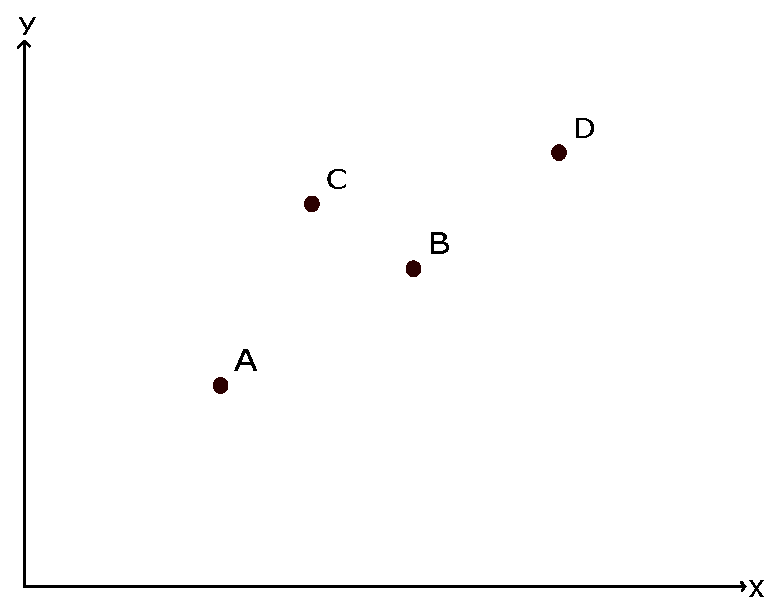
\includegraphics[scale=0.5]{Capitulo2/assets/dominancia.eps}
	\centering
	\caption{Ejemplo de dominancia y �ptimo de Pareto}
	\label{fig:dominancia}
\end{figure}

\subsubsection{Frontera de Pareto}

\label{sec:frontera_pareto}
La frontera de Pareto es el conjunto de todas las soluciones no dominadas las cuales componen las soluciones �ptimas al problema multiobjetivo. En la Figura~\ref{fig:frente_pareto} los puntos rojos componen la frontera de Pareto.

\begin{figure}[h]
	 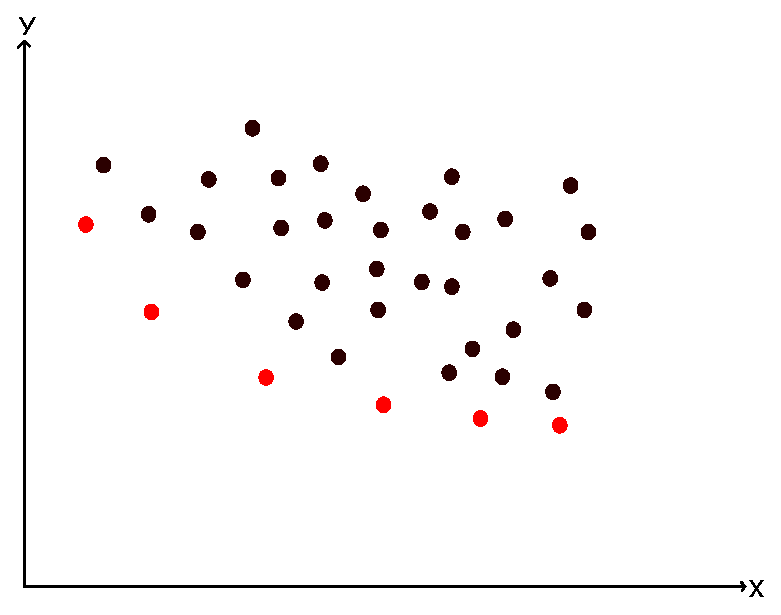
\includegraphics[scale=0.5]{Capitulo2/assets/frontera-pareto.eps}
	\centering
	\caption{Ejemplo frente de Pareto}
	\label{fig:frente_pareto}
\end{figure}

